\documentclass[tikz,border=4pt]{standalone}

\usepackage{fontspec}
\usepackage{unicode-math}
\usepackage{pgfplots}
\usepgfplotslibrary{groupplots}

\pgfplotsset{compat=1.18}

% Compile with LuaLaTeX or XeLaTeX.
\setmainfont{STIX Two Text}
\setmathfont{STIX Two Math}

\pgfplotsset{
  minifem axis/.style={
      width=15.5cm,
      height=6.0cm,
      xmin=0,
      xmax=1000,
      xtick={0,250,500,750,1000},
      grid=both,
      major grid style={draw=gray!35,dashed,line width=0.4pt},
      minor grid style={draw=none},
      axis line style={line width=0.8pt},
      tick style={line width=0.8pt},
      tick align=outside,
      tick label style={font=\small},
      label style={font=\normalsize},
      title style={font=\normalsize,anchor=west},
      legend style={
          draw=none,
          fill=none,
          font=\small,
          cells={anchor=west},
        },
      clip=false,
    }
}

\begin{document}

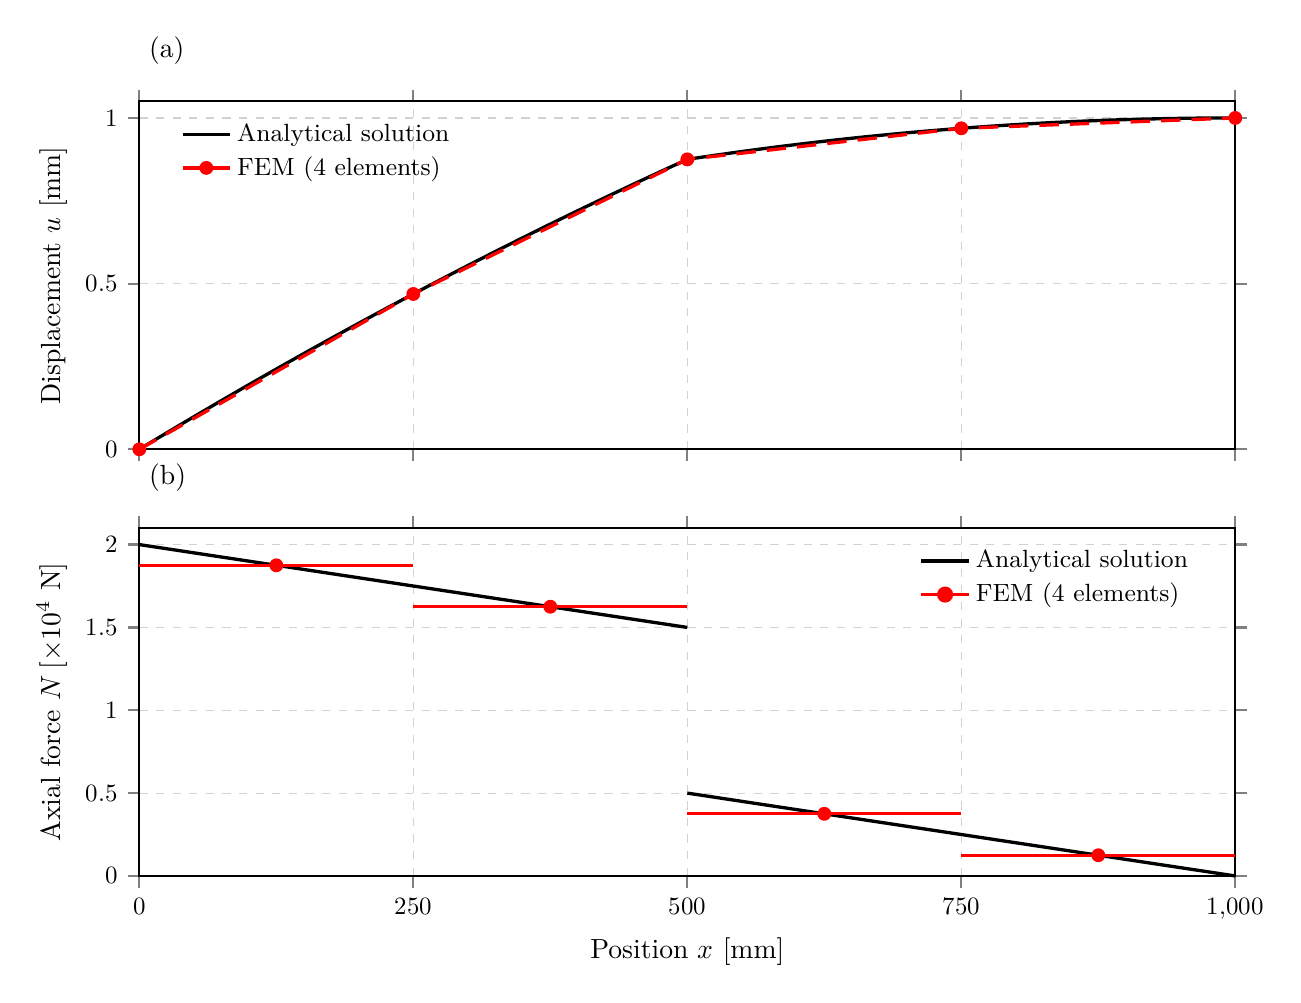
\begin{tikzpicture}

  \begin{groupplot}[
      group style={
          group size=1 by 2,
          vertical sep=1.0cm,
          xlabels at=edge bottom,
        },
      minifem axis,
    ]

    % ------------------------------------------------------------------
    % (a) Displacement
    % ------------------------------------------------------------------
    \nextgroupplot[
      ymin=0,
      ymax=1.05,
      ylabel={Displacement \(u\) [mm]},
      title={(a)},
      title style={at={(axis description cs:0,1.03)},anchor=south west},
      legend pos=north west,
      xticklabels=\empty,
    ]

    % Analytical solution, 0 <= x <= 500 mm
    \addplot[
      black,
      line width=1.2pt,
      domain=0:500,
      samples=120,
      forget plot,
    ]
    {(10*(1000*x - x^2/2) + 10000*x)/1e7};

    % Analytical solution, 500 <= x <= 1000 mm
    \addplot[
      black,
      line width=1.2pt,
      domain=500:1000,
      samples=120,
      forget plot,
    ]
    {(10*(1000*x - x^2/2) + 10000*500)/1e7};

    % FEM nodal displacement interpolation:
    % draw the dashed line separately from the nodal markers
    \addplot[
      red,
      dash pattern=on 7pt off 4pt,
      line width=1.2pt,
      forget plot,
    ]
    coordinates {
        (0,0)
        (250,0.46875)
        (500,0.875)
        (750,0.96875)
        (1000,1.0)
      };

    % FEM nodal markers: uniform filled circular dots
    \addplot[
      only marks,
      red,
      mark=*,
      mark size=2.3pt,
      forget plot,
    ]
    coordinates {
        (0,0)
        (250,0.46875)
        (500,0.875)
        (750,0.96875)
        (1000,1.0)
      };

    % Explicit legend entries
    \addlegendimage{
      black,
      solid,
      line width=1.2pt
    }
    \addlegendentry{Analytical solution}

    \addlegendimage{
      legend image code/.code={
          \draw[
            red,
            dash pattern=on 7pt off 4pt,
            line width=1.2pt
          ] (0cm,0cm) -- (0.6cm,0cm);
          \fill[red] (0.3cm,0cm) circle[radius=2.3pt];
        }
    }
    \addlegendentry{FEM (4 elements)}

    % ------------------------------------------------------------------
    % (b) Axial force
    % ------------------------------------------------------------------
    \nextgroupplot[
      ymin=0,
      ymax=2.1,
      xlabel={Position \(x\) [mm]},
      ylabel={Axial force \(N\) [\(\times 10^{4}\) N]},
      title={(b)},
      title style={at={(axis description cs:0,1.03)},anchor=south west},
      legend pos=north east,
    ]

    % Analytical solution, left of the point load
    \addplot[
      black,
      line width=1.2pt,
      domain=0:500,
      samples=120,
      forget plot,
    ]
    {(10*(1000-x) + 10000)/1e4};

    % Analytical solution, right of the point load
    \addplot[
      black,
      line width=1.2pt,
      domain=500:1000,
      samples=120,
      forget plot,
    ]
    {(10*(1000-x))/1e4};

    % FEM piecewise-constant axial force:
    % horizontal segments only, with no vertical jump lines
    \addplot[
      red,
      solid,
      line width=1.2pt,
      forget plot,
    ]
    coordinates {
        (0,1.875)
        (250,1.875)
      };

    \addplot[
      red,
      solid,
      line width=1.2pt,
      forget plot,
    ]
    coordinates {
        (250,1.625)
        (500,1.625)
      };

    \addplot[
      red,
      solid,
      line width=1.2pt,
      forget plot,
    ]
    coordinates {
        (500,0.375)
        (750,0.375)
      };

    \addplot[
      red,
      solid,
      line width=1.2pt,
      forget plot,
    ]
    coordinates {
        (750,0.125)
        (1000,0.125)
      };

    % FEM element midpoint values: uniform filled circular dots
    \addplot[
      only marks,
      red,
      mark=*,
      mark size=2.3pt,
      forget plot,
    ]
    coordinates {
        (125,1.875)
        (375,1.625)
        (625,0.375)
        (875,0.125)
      };

    % Explicit legend entries
    \addlegendimage{
      black,
      solid,
      line width=1.2pt
    }
    \addlegendentry{Analytical solution}

    \addlegendimage{
      red,
      solid,
      line width=1.2pt,
      mark=*,
      mark size=2.3pt
    }
    \addlegendentry{FEM (4 elements)}

  \end{groupplot}

\end{tikzpicture}

\end{document}
